\chapter{Related Work}
\label{chap:related}

\par The field of computer vision has evolved from natural vision. Its main purpose is to allow machines to understand visual information based on the natural way humans gain information from visual input.
\par This branch of computer science is widely used to gain insight into the real world through different algorithms and computational techniques, solving problems such as object detection in an image or video, scene understanding and image generation. The solutions from this field open the door for new innovations, which can be seen in the everyday life in the form of image filters, self-driving cars and so on.
\par The evolution of computer vision can easily be followed along with the evolution of computational power, given the high requirements of image processing. In the earlier days, such as the 1960s and 1970s, the first algorithms were very limited by the processing power available. As time passed, more sophisticated ones were created, such as Hough Transform, the Viola-Jones face detection and machine learning.

\begin{figure}
    \centering
    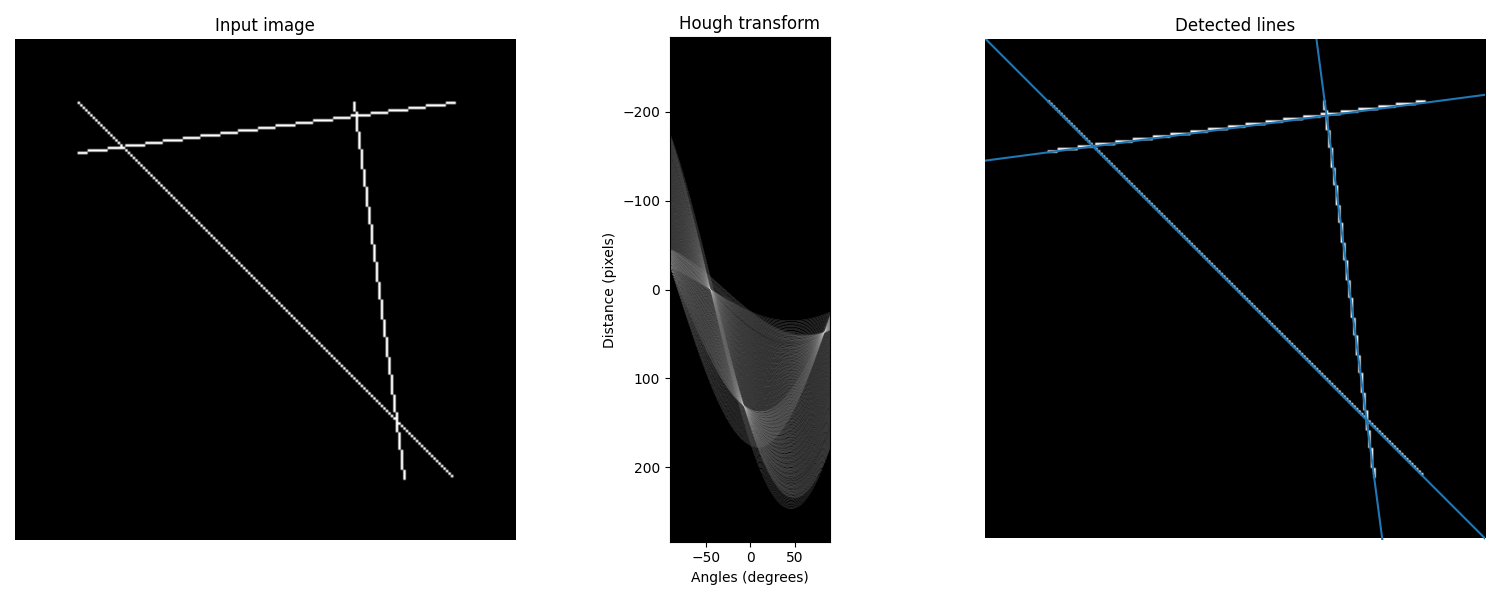
\includegraphics[width=0.5\linewidth]{figures/HoughTransform.png}
    \caption{Hough transform calculation to find the lines of a triangle \cite{hough}}
    \label{fig:houghl}
\end{figure}

\section{Image segmentation algorithms}
\label{sec:relatedsec1}

\subsection{Hough Transform}
\label{subsec:relatedsec1subsec1}

\par This technique was proposed by Paul Hough in 1962, as a method to identify patterns in images. \cite{Duda1972}
\par The core idea behind it is a voting process made by the curves in the transform space, creating cluster points or local maxima, which represents the existence of a shape since the curves contain the parameters of it. From those parameters the position of the shape in the input image can be detected, shown in Figure \ref{fig:houghl}.
\par The main strength of this method is that it is capable of identifying shapes even in slightly obscured or noisy data, which made this procedure a massive breakthrough in image processing. It is used in many sectors, from robotic navigation, by identifying edges and lines in the environment, to medical imaging, by detecting circular shapes potentially depicting different biological conditions and many more, where image processing can be utilized.

\subsection{Viola-Jones Face Detection}
\label{subsec:relatedsec1subsec2}
\par Another breakthrough in computer vision was the face detection procedure proposed by Paul Viola and Michael Jones in 2001 \cite{viola2001}. Their approach being based on the usage of Haar-like feature and Adaptive Boosting.
\par The Haar-like features are simple rectangular regions in the input image data, which are being used for decreasing the number of pixel calculations and for getting a better understanding of a specific region. By calculating the differences in the sum of pixel intensities between the regions, the contrast can be learned, which allows the detection of basic patterns, like edges, lines and textures.
\par Adaptive boosting is a machine learning algorithm used for enhancing weak classifiers, by training the model in iterations, focusing on one feature each time. At each pass, the algorithm selects the best performing classifier and merges it with the final one, with a weight proportional to its performance. By increasing the weight of incorrect classifications for the next step, it achieves a dynamically changing priorities, boosting the model even more.
\par With the help of these two procedures this method achieves great accuracy in real-time, more specifically at 15 frames per second on a 700 MHZ Intel Pentium III, using approximately 50 thousand parameters. Because of its low requirements it is still widely used on weaker devices.

\section{Deep learning algorithms}
\label{sec:relatedsec2}
\par With the increase in computational power, image processing algorithms have also evolved in tandem. As seen in the Viola-Jones face detection algorithm, machine learning were already used in the early 2000s, be it at a smaller scale. As more power machines become available the parameters used in these techniques increased accordingly, allowing the learning of more complex features. In this section I choose some deep learning architectures, which were significant achievements, and are still in use today.

\subsection{YOLO}
\label{subsec:relatedsec2subsec1}
\par YOLO (You only live once) is an object detection method, based on a Convolutional Neural Network backbone, the building blocks of which can be seen in Table \ref{YoloTable}, containing convolutional layers of varying sizes.
\par The main selling point of this algorithm is that it achieves real-time performance with a single-pass approach. It divides the image into a grid, each predicting a bounding box, with an associated confidence score and class probability. Utilizing these values and various anchor boxes, which are bounding boxes with a predefined shape, size and aspect ratio, the model predicts the final bounding box for the searched object. \cite{redmon2018yolov3}
\par Since its real-time performance the method has been utilized in many projects, from autonomous driving to surveillance systems.

\begin{table}[htbp]
\begin{center}
\begin{tabular}
{|p{90pt}|p{90pt}|p{90pt}|p{90pt}|}
\hline
 Type  &  Filters & Size & Output\\
\hline 
\hline Convolutional & $64-1024$ & $3x3/2$ & $128x128-8x8$ \\
\hline Convolutional & $32-512$ & $1x1$ & $ $ \\
\hline Convolutional & $64-1024$ & $3x3$ & $ $ \\
\hline Residual & $ $ & $ $ & $128x128-8x8$ \\
\hline
\end{tabular}
\end{center}
\caption{Building blocks for the YoloV3 CNN backbone, Darknet-53 \cite{redmon2018yolov3}}
\label{YoloTable}
\end{table}

\subsection{RESNET}
\label{subsec:relatedsec2subsec2}
\par ResNet is a convolutional neural network proposed by Kaiming He and co. in 2015, achieving great performances in various computer vision tasks.
\par The main strength of this model comes from addressing the vanishing gradient problem, via the introduction of skip connections. The residual blocks, the main building blocks of this model, contain the shortcut connections, skipping one or more layers. This allows the network to be able to learn on a much larger scale compared to previous designs, by being able to increase the depth without the gradient vanishing. \cite{he2015deep}
\par As can be seen in Table \ref{ResNetTable}, the complexity of this model can grow to incredible levels, containing as much as 19.7 million parameters, although in those cases the hardware requirements can also get out of hand.

\begin{table}[htbp]
\begin{center}
\begin{tabular}
{|p{120pt}|p{120pt}|}
\hline
Number of layers & Number of parameters\\
\hline 
\hline $20$ & $0.27M$ \\
\hline $32$ & $0.46M$ \\
\hline $44$ & $0.66M$ \\
\hline $56$ & $0.85M$ \\
\hline $110$ & $1.7M$ \\
\hline $1202$ & $19.7M$ \\
\hline
\end{tabular}
\end{center}
\caption{Correlation between the size of the model and the number of parameters used \cite{he2015deep}}
\label{ResNetTable}
\end{table}

\subsection{MOBILENET}
\label{subsec:relatedsec2subsec3}
\par MobileNet is a convolutional neural network designed for reasonable performance on limited hardware.
\par The architecture is built using two techniques: the depth-wise and point-wise convolutions. In the first one a single convolution filter is applied for each input channel, capturing features separately, while the second applies a 1x1 filter to the outputs of the the previous calculations, combining the results. This allows the model to significantly reduce the number of parameters needed, compared to normal convolution, thus decreasing the computational power needed. \cite{howard2017mobilenets}
\par In table \ref{MobileNetTable} the difference between the complexity of the two architectures can be seen, tested on the ImageNet dataset, trading around 1 percent accuracy for around seven times less parameters, greatly decreasing the computational quantity.

\begin{table}[htbp]
\begin{center}
\begin{tabular}
{|p{120pt}|p{120pt}|p{120pt}|}
\hline
Model & ImageNet Accuracy & Parameters\\
\hline 
\hline Conv MobileNet & $71.7\%$ & $29.3M$ \\
\hline MobileNet & $70.6\%$ & $4.2M$ \\
\hline
\end{tabular}
\end{center}
\caption{Difference in parameters between the two method and fully convolutional MobileNet architectures \cite{howard2017mobilenets}}
\label{MobileNetTable}
\end{table}